\documentclass[journal,twoside]{JoPhA}

\usepackage{color}
\usepackage{flushend}

\usepackage[pdftex]{graphicx}
% declare the path(s) where your graphic files are
\graphicspath{{figures/}}
% and their extensions so you won't have to specify these with
% every instance of \includegraphics
\DeclareGraphicsExtensions{.pdf,.jpeg,.png}

\begin{document}

\title{Cybersecurity in Autonomous Systems: Evaluating the performance of hardened ROS}

\author{David Ma\~nanes, Francisco Javier Rodr\'iguez Lera, Jes\'us Balsa and Vicente Matell\'an,
\IEEEcompsocitemizethanks{
All authors are with the Robotics Group (http://robotica.unileon.es) and the Research Institute on Applied Sciences to Cybersecurity (http://riasc.unileon.es) at Universidad de Le\'on (Spain).

\IEEEcompsocthanksitem Corresponding author: vicente.matellan@unileon.es} % <-this % s
}


\markboth{Workshop on Physical Agents, M\'alaga 2016}%
{Matell\'an et al: Cybersecurity in ROS}
\maketitle


\begin{abstract}
As robotic systems spread, cybersecurity emerges as major concern. Currently most research autonomous systems are built using the ROS framework, along with other commercial software. ROS is a distributed framework where nodes publish information that other nodes consume. This model simplifies data communication but poses a major threat because a malicious process could easily interfere the communications, read private messages or even supersede nodes. In this paper we propose that ROS communications should be ciphered. We also measure how this ciphering affects its performance. We have used three different ciphering techniques: DES, AES and RSA. We have evaluated the performance of the system, both from the computing and the communications points of view. Preliminary results show that symmetric ciphers using private keys impose significant delays.

\end{abstract}


\begin{IEEEkeywords}
autonomous systems, cybersecurity, robotics, performance, cyber-physical systems, ciphers
\end{IEEEkeywords}


\section{Introduction}

\IEEEPARstart{A}{utonomous} systems are spreading not just in the virtual world (Internet, software systems), or in science-fiction movies, but in our ordinary real world. Currently we can find driverless cars in the streets, autonomous vacuum cleaners in our homes, museum guides, hotel assistants, etc. These cyber-physical systems, as any computer-based system, can suffer different types of vulnerabilities, and the need of cybersecurity \cite{Morante2015} is required. 

ROS (Robotic Operating System) \cite{ROS09} has become the most popular framework for developing robotic applications. It started in the research environment, but currently most of manufacturers of commercial platforms use ROS as the {\em de facto} standard for building robotic software. For example, object-manipulation robots like Baxter (by Rethink robotics){\textcolor{red}{[poner REF]}} or service robots as our RB1 (by Robotnik){\textcolor{red}{[poner REF]}} are ROS based platforms.

Our research group is developing assistant robot~\cite{Martin2014} for the elderly. When we initiated experiments involving potential users, caregivers have asked us about the security of our robot, and about the privacy of its communications \cite{Denning2009}. If an assistant robot carrying a camera is deployed in a home, the access to the camera should be secured. Even more when the robot is managing medical information. We have developed all our software for the autonomous behaviour of the robots using ROS, so we need to consider its security.


\subsection{ROS security assestment}

ROS provides specific libraries for robotics as well as classical operating system services such as hardware abstraction (for sensors and actuators), low-level device control, and inter-process communication. Inter-process communication is based on a graph architecture where computation takes place in ROS processes named nodes. These nodes can receive and send messages, but no security was considered in its design. 

ROS framework is basically a message-passing distributed system. Its architecture is based on processes that publish {\em messages} to {\em topics}. For instance, a process ({\em node}) can be in charge of accessing a sensor, making the basic processing of the information, and publishing it as a structure information on a named topic. Another process can {\em subscribe} to this topic, that is, it can read that information, make a decision about the movement of the robot. These commands will be sent to the motors in another topic. These nodes can be running in the same computer or in different computers. 

This approach is very convenient for developers but it is very easily tampered by malicious hackers. For instance in \cite{McClean2013} an experiment involving a ROS-based honeypot is described. The honeypot was a radio model truck with two cameras and a compass as sensors and controlled from a remote ROS node written in Javascript and hosted in a remote enterprise grade web server. Vulnerabilities described in the paper range from plain-text communications, unprotected TCP ports to unencrypted data storage.

These vulnerabilities are a subset of the security problems threatening any computing system:
{\textcolor{red}{No s\'e si merece la pena, demasiado generalista. Igual es mejor hablar más de cosas específicas de robótica y de ROS en particular}}
\begin{enumerate}
 \item Availability: Interruption
 \item Confidenciatily: Interception
 \item Integrity: Modification
 \item Authenticity :Fabrication
\end{enumerate}

Figure \ref{fig:Conceptualmodel} graphically summarizes these problems in our robot.

\begin{figure}[ht]
    \centering
    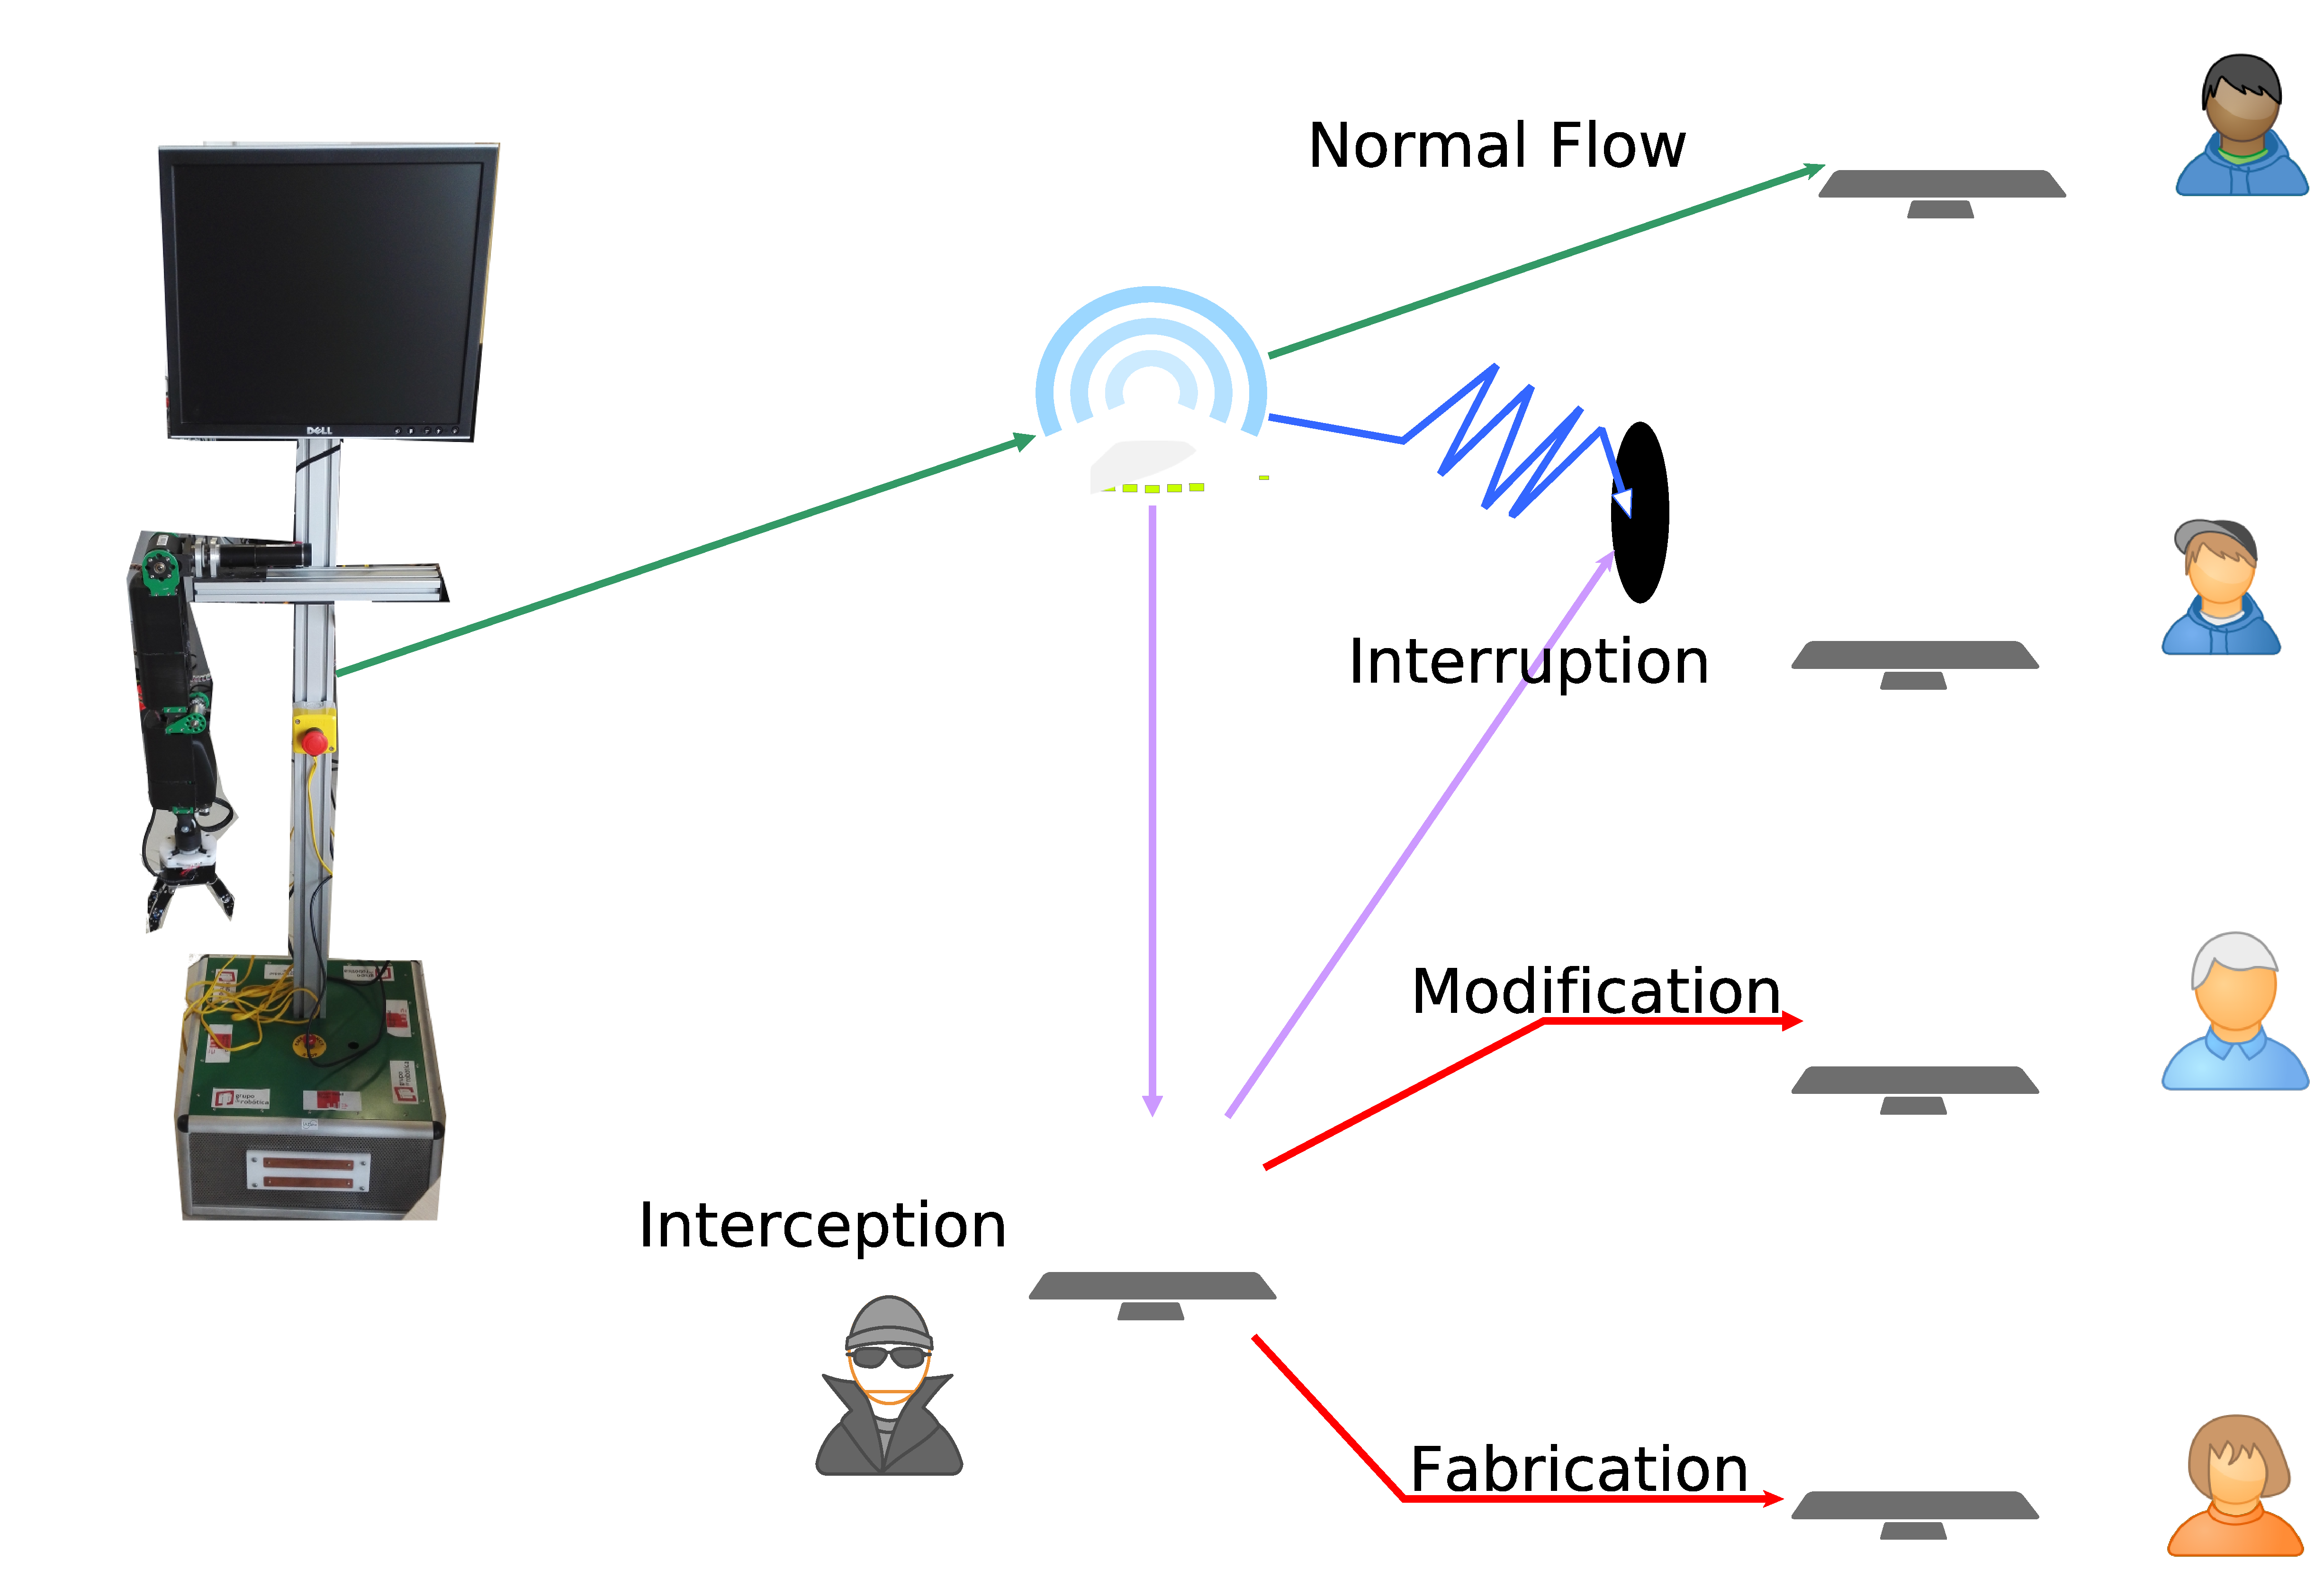
\includegraphics[width=.5\textwidth]{SecurityAttacks.pdf}
    \caption{Conceptual model of the security attacks.}
  \label{fig:Conceptualmodel}
\end{figure}

The first step to solve some of these problems is to secure the communication channels by using a ciphering mechanism. but, how does this systems impact on the performance of a robotic system? This is the goal of this paper, characterize and evaluate different alternatives to secure ROS communication mechanism.

Next section describes the testbed we have designed to measure the performance of the encrypted ROS system. Third section evaluates the data obtained in the experiments and in the last section some conclusions and further work are presented.



\section{Testbed description}

We want to evaluate whether ciphering communications would affect the performance of ROS. 


\subsection{Simulated testedbed}

We have installed ROS Jade in two computers connected through a wired Ethernet 10/100 switch (model XXXX). In the first computer we have connected a Xtion camera and a Hokuyo laser. In the second computer have run a node visualizing the information from the sensors. Figure \ref{fig:maqueta} shows this environment.


Then we modified the standard ROS implementation. We changed the TCP/IP sockets based implementation by ciphered ones.


\subsection{Robotic testbed}

In the second experiment we changed the first computer for a RB1 robot and the XXX switch by a wireless one. This robot was also running ROS Jade.



\section{Experimental Measuments}




Figure \ref{fig:velocidad-maqueta} shows the maximum rate that can be reached both in the laser and the camera visualization according to \texttt{rviz} information.

The same measurements were made in the second environment to see if the use of wireless systems and a real robot would have any influence.

The absolute values of the frame rates is obviously different, as shown in figure \ref{fig:velocidad-robot}. But the interesting part is the relative different when using clear communications or ciphered ones. 

Table \ref{tab:relativas}  compares the relative reduction of speed when using ciphered protocols vs clear ones in both environments as well as the relative increase of CPU usage.

We have addded a funtion to our program in order to measure the time spent in each encrypt and decrypt call. The function is a python method presented as a decorator pattern 

{
  \footnotesize{
    \begin{verbatim}
def fn_timer(function):
	  @wraps(function)
	  def function_timer(*args, **kwargs):
	      v_time_0 = time.time()
	      result = function(*args, **kwargs)
	      v_time_1 = time.time()
	      return result
	  return function_timer
    \end{verbatim}
  }
}

\begin{figure*}[ht]
    \centering
    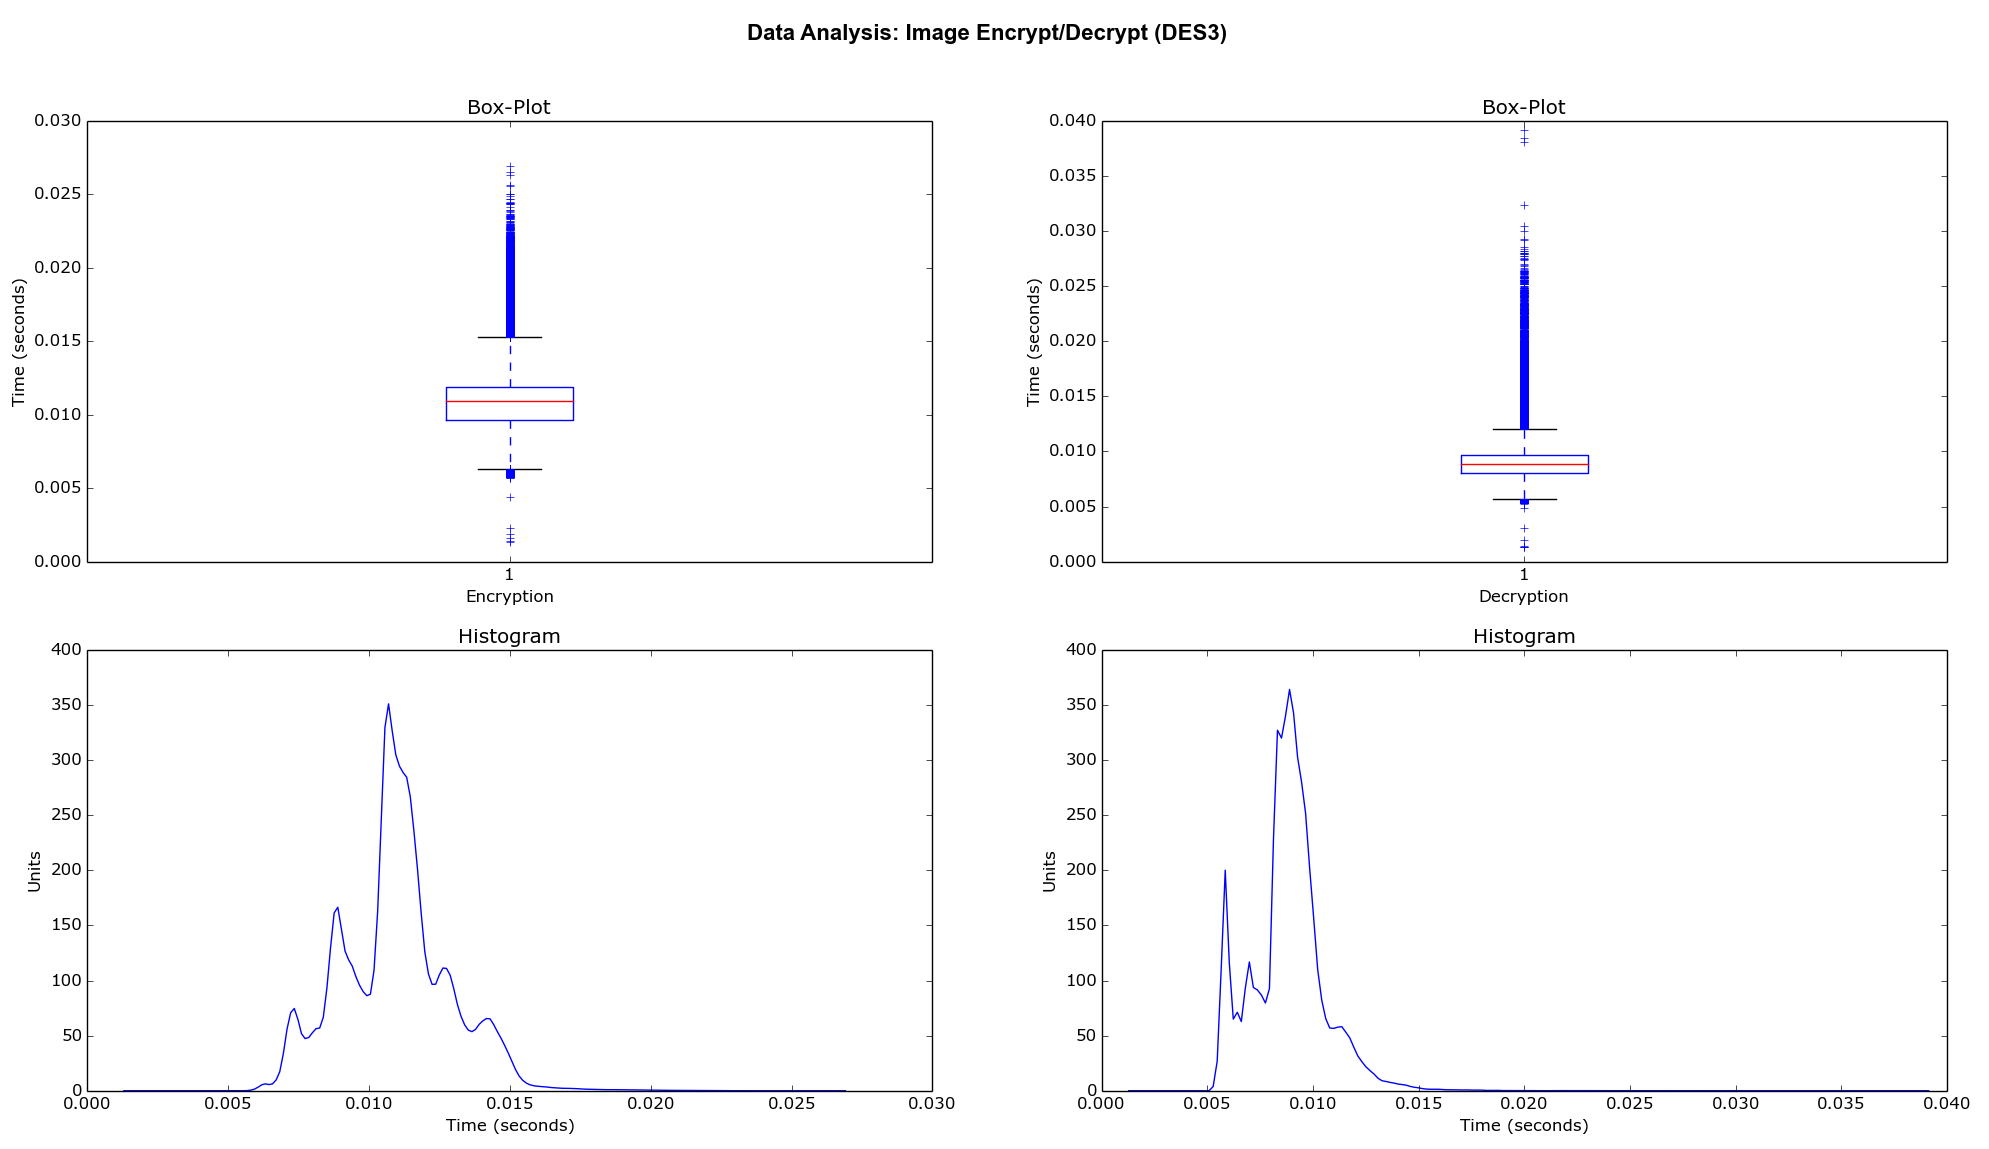
\includegraphics[width=.9\textwidth]{Resumen_llamada_funcion.png}
    \caption{Time spent in each call to encryption/decryption function.}
  \label{fig:Conceptualmodel}
\end{figure*}


\subsection{Camera}
Encrypt

PC: 234 process

Total length 971790 frames, min time 0.001309 seconds, max time  0.026909
Cifrado mean: 0.010948
Cifrado stdev: 0.000004
El valor moda de la fase de cifrado fue:
(array([ 0.010571]), array([ 415.]))

Descifrado length: 969295.000000
Descifrado min: 0.001288
Descifrado max: 0.039130
Descifrado mean: 0.008828
Descifrado stdev: 0.000003
El valor moda de la fase de descifrado fue:
(array([ 0.008183]), array([ 593.]))


PC descifrador: 242 process (ps -ef | wc -l)

Cifrador
[INFO] Encrypter node:  elasped time: 66755.17
[INFO] Encrypter node:  approx. FPS: 14.56



Descifrador
[INFO] Decrypter node: elapsed time: 66659.74
[INFO] Decrypter node: approx. FPS: 14.54



\begin{figure}[ht]
    \centering
    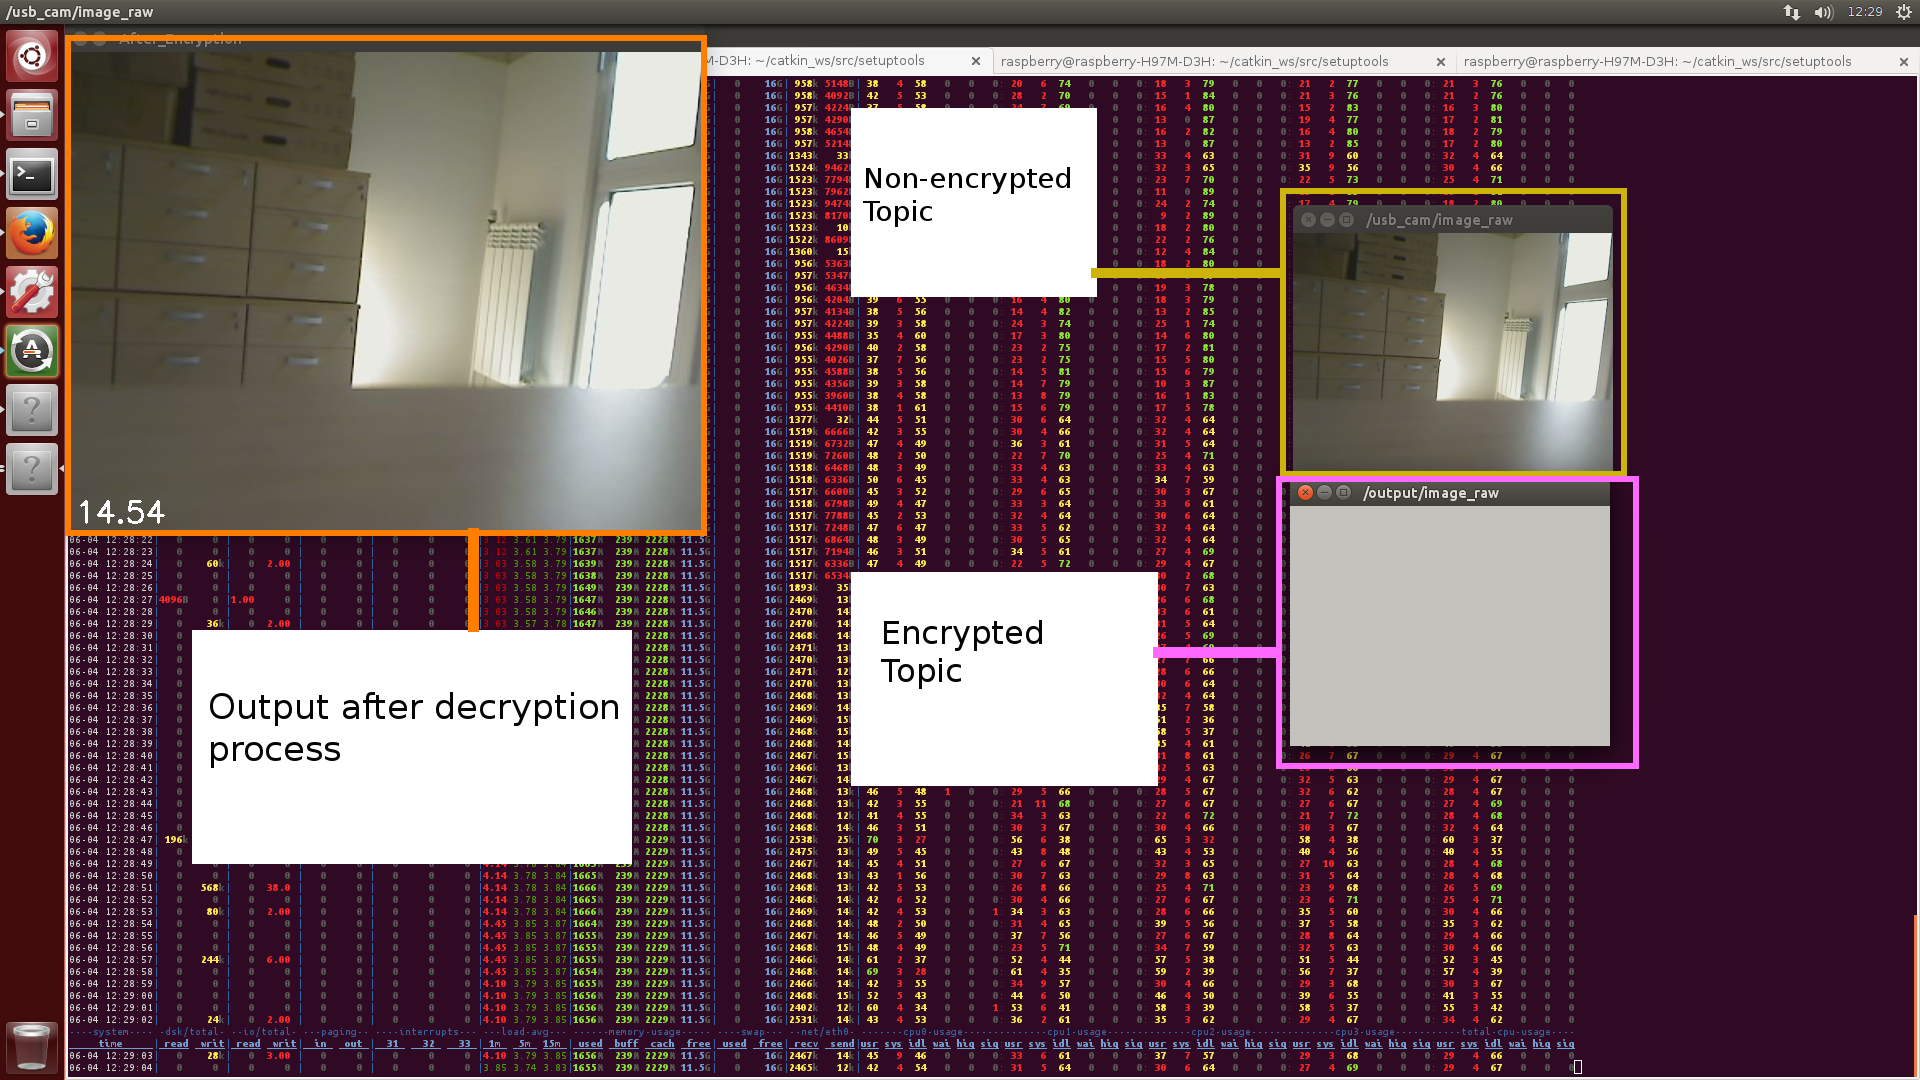
\includegraphics[width=.5\textwidth]{Screenshot.png}
    \caption{Time spent in each call to encryption/decryption function.}
  \label{fig:Conceptualmodel}
\end{figure}




\section{Conclusion and Futher Work}

We have evaluated the influence of cyphering in the performance of ROS based robotic systems.

As we commented in the introduction, we think that securing communications is just one dimension in  the cybersecurity of Autonomous Systems. If we want to see autonomous systems working in our homes we need to secure the navigation abilities, the interaction mechanisms, etc. 
 
Some works have been sketched in this area, as for instance in \cite{Guiochet2016}.




\section*{Acknowledgment}
The authors would  like to thank the Spanish Ministry of Economy and Competitiveness for the partial support to this work under grant DPI2013-40534-R and to the Spanish National Institue of CyberSecurity (INCIBE) under grand Adenda21 ULE-INCIBE.

\bibliographystyle{plain} 
\bibliography{waf2016}

\end{document}


